\chapter{Microsoft Azure}
\begin{comment}
Introduction
Quick Start
Fundamentals
  Architecture
  Service Management
Examples
  Login
  Azure VM
Conclusions
\end{comment}
In questi capitoli sarà presentato Azure, il cloud provider di Microsoft, cercando di affrontare aspetti generici dell'architettura ed esempi specifici. Azure, come tutti i cloud provider, è in perenne evoluzione e quindi risulta difficile possedere una conoscenza specifica di tutti i servizi che offre: Microsoft infatti mette a disposizione dei corsi per ottenere certificazioni di utilizzo del proprio provider. Lo scopo di questi capitoli è cercare di ottenere una visione d'insieme di tutta la piattaforma e delle tecnologie che attualmente Azure mette a disposizione, e di fare pratica su alcuni esempi specifici.

Il materiale utilizzato dalle lezioni del prof. e in questi appunti è presente sulla piattaforma elearning di ateneo.

\section{Introduzione}
Azure è una piattaforma Cloud completa che permette di ospitare le applicazioni, gestire lo sviluppo e migliorare il rendimento delle risorse on-premise. Integra i servizi cloud necessari a sviluppare, testare e distribuire le applicazioni, ed ha come obiettivo quello di rendere possibile la scalabilità in base alle richieste dei cloud consumer. Azure offre la reliability necessaria a far sì che le applicazioni siano sempre disponibili e che siano funzionali in diverse regioni, il tutto grazie ad una gestione semplificata attraverso il portale web, ma anche attraverso le API e i template.

\vspace{5mm}

Azure offre diversi tipi di servizi che supportano lo sviluppo in qualsiasi direzione, coprendo quindi tutti i possibili modelli di deployment, da IaaS a FaaS (Function as a Service).

\begin{figure}[htb!]
    \centering
    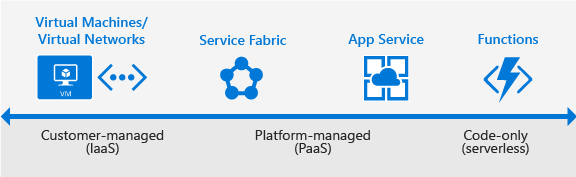
\includegraphics[width=12cm]{./Images/cap14/14.1.png}
\end{figure}

\begin{itemize}
    \item Con IaaS è possibile ottenere il massimo del controllo sull'hosting dell'applicazione hostata su Azure;. Per quanto riguarda l'application hosting, è possibile fare il deploy di ambienti Windows e Linux, ed è possibile configurare la rete per supportare l'hosting di macchine virtuali Windows e Linux. Con IaaS è possibile configurare qualsiasi aspetto della VM: tutte le installazioni di software, manutenzione del sistema operativo e delle patch di sistema devono essere effettuate manualmente. È possibile scegliere tra diversi servizi di server workload su Azure: database, Windows Server Active Directory e Microsoft SharePoint. \textbf{Azure Service Fabric} è una piattaforma distribuita che permette di realizzare con facilità l'intero ciclo di vita di un microservizio (build, package, deploy, gestione). Fornisce anche degli strumenti di gestione per il monitoring, l'aggiornamento e il patching delle applicazioni pubblicate. Il vantaggio di queste app è che è molto facile scalare in quanto sono in esecuzione su pool condivisi. Service Fabric supporta le WebAPI con interfaccia Open Web per .NET e ASP.NET Core e diversi SDK per costruire servizi su Linux sia in .NET che in Java. 
    \item PaaS offre tutti i servizi necessari per far funzionare l'applicazione. Il vantaggio di Azure è l'integrazione con gli ambienti di sviluppo di Microsoft e con il sistema operativo e gli strumenti di Microsoft. \textbf{Azure App Service} è la maniera più semplice per pubblicare progetti web-based su REST API, fornisce l'autenticazione tramite social provider (Google, Facebook) e tutta una serie di feature per l'auto scaling, oltre che a strumenti per il testing in produzione e strumenti di supporto come ambienti di deployment basati su container. È possibile lavorare a tutti i livelli, quindi creare webapps, backend di applicazioni moble o semplici API. Dato che tutti e tre i tipi di applicazioni condividono l'App Service Runtime, uno stesso progetto può gestire un sito web, supportare client mobile oppure esporre le proprie API su Azure. App Service è pensato per funzionare nativamente con DevOps, quindi offre supporto alle webhooks di GitHub, Jenkins, Azure DevOps, TeamCity e altri.
    \item FaaS pernette l'esecuzione di codice in maniera efficiente e scalabile. Con Azure è possibile anche mettere su cloud solamente delle funzioni scritte in un certo linguaggio, ed evocarle in seguito a trigger o eventi, come richieste HTTP, webhooks o cloud service events, secondo il "serveless style". I linguaggi supportati sono C\#, F\#, Node.js, Python o PHP. Il serveless si paga solamente per il tempo di utilizzo.
\end{itemize}

In aggiunta all'hosting di applicazioni Azure mette a disposizione diversi servizi che migliorano il ciclo di vita di un'applicazione, tra cui:
\begin{itemize}
    \item Accesso a storage e dati
    \item Supporto a Docker
    \item Autenticazione
    \item Monitoring (Pay-Per-Use Monitor, Audit Monitor, ecc.)
    \item Integrazione con DevOps
\end{itemize}

\subsubsection{\textbf{ACCESSO A STORAGE E DATI}}
Riguardo questa tipologia di servizi viene offerto \textbf{Azure Cosmos DB}: un database multimodello capace di scalare in maniera molto ampia su diverse regioni con un SLA estremamente ricco di vincoli che garantiscono l'affidabilità e le prestazioni di questo database. \textbf{Azure Storage} offre invece servizi di archiviazione per blob, oggetti e file non relazionali, e viene utilizzato per le VM. \textbf{Azure SQL Database} invece è una versione di Microsoft SQL Server basata su Azure per salvare dati in forma tabulare sul cloud con tutti i suoi benefici che conosciamo (prestazioni, scalabilità, no downtime e protezione dei dati). Il \textbf{Data Factory} di Azure permette di portare sul cloud le risorse on-premise o collegare i servizi presenti sul cloud con le risorse on-premise.

\subsubsection{\textbf{SUPPORTO A DOCKER}}
Un'applicazione \textit{containerizzata} lavora allo stesso modo in sviluppo, in test e in produzione, questo grazie ai Docker tools. Azure mette a disposizione la \textbf{Docker VM extension} che permette di configurare una macchina virtuale con gli strumenti di Docker per renderla pronta per funzionare come un host. \textbf{Azure Container Service} serve invece a creare, configurare e gestire un cluster di macchine virtuali preconfigurate per eseguire applicazioni basate su container. \textbf{Docker Machine} serve a installare e gestire un Docker Engine su macchine virtuali utilizzando una linea di comando. Il servizio che permette di ottenere file immagine di un Docker container e pubblicare l'immagine su Linux è \textbf{Custom Docker image for App Service}.

\subsubsection{\textbf{AUTENTICAZIONE}}
Per quanto riguarda l'autenticazione \textbf{Azure Active Directory} è il prodotto di punta di Microsoft, che fornisce servizi per autenticazione, controllo degli accessi e identità cloud. Con Azure AD è possibile aggiungere il Single-Sign On (SSO) alle applicazioni, grazie all'integrazione con provider esterni come OAuth 2.0, Open ID Connect e endpoint nativi HTTP/REST. Il supporto all'autenticazione nativo di Azure AD è chiamato \textbf{App Service Authentication}, e fornisce possibilità di autenticarsi con diversi provider, tra i quali ci sono Facebook, Google, Microsoft e Twitter. 

\subsubsection{\textbf{MONITORING}}
Una delle cose più importanti che aumentano la qualità del servizio è l'integrazione di Azure con gli ambienti di sviluppo e in particolare con Visual Studio, grazie a \textbf{Visual Studio Application Insights}, che permette di monitorare tutte le componenti di applicazioni che riguardano progetti web-based e non solo. Grazie ad \textbf{Azure Monitor} è possibile visualizzare, gestire, archiviare e controllare le metriche e i log che sono generati dall'infrastruttura e dalle risorse. 

\subsubsection{\textbf{INTEGRAZIONE CON DEVOPS}}
Azure fornisce l'integrazione con i più popolari strumenti per DevOps, come Jenkins, GitHub, Puppet, Chef, TeamCity, Ansible, Azure DevOps. Uno degli aspetti classici di Azure è fornire gli standard di riferimento ma fornire anche gli strumenti proprietari. 

\subsection{Regioni}
Azure è disponibile in 54 regioni in tutto il mondo (2019). Quando un servizio/macchina virtuale/applicazione viene sviluppata sul cloud, è possibile selezionare una regione, che rappresenta lo specifico centro di calcolo (data center) dove l'applicazione sarà ospitata, così come i dati. Una regione è un insieme di centri di calcolo distribuiti in un perimetro definito in base alla velocità di connessione e connessi tramite una rete regionale a bassa latenza.

Una zona geografica (Geography) contiene due o più regioni che preservano la residenza dei dati e limiti di conformità. Sono molto utili per utenti con specifici vincoli di consistenza e residenza dei dati oppure che vogliono semplicemente che i propri dati siano ospitati in una regione vicina. Le zone geografiche sono resistenti ai fallimenti della regione in cui si trovano grazie a un'infrastruttura basata su connessioni ad alta velocità. Le \textbf{Availability Zones} sono posizioni separate fisicamente all'interno di una regione. Ogni AZ è composta da più datacenter provvisti di corrente elettrica indipendente, sistemi di raffreddamento e infrastrutture di rete, per permettere ad applicazioni critiche di poter funzionare sempre e comunque grazie ad un'alta availability e a una replicazione dei dati a bassa latenza.

\begin{figure}[htb!]
    \centering
    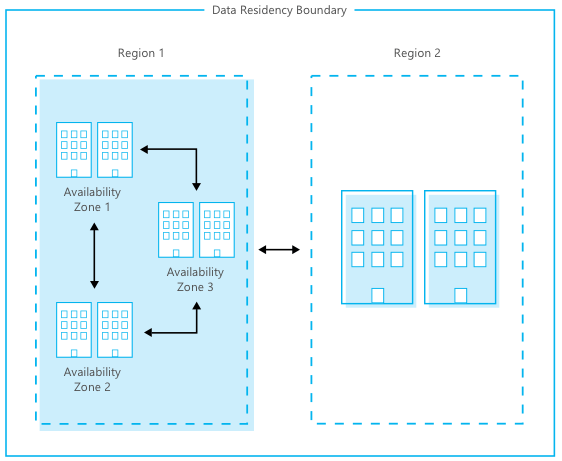
\includegraphics[width=8cm]{./Images/cap14/14.2.png}
\end{figure}

Un importante vantaggio nell'utilizzo di Azure è quello di poter pubblicare le applicazioni in diversi datacenter contemporaneamente. La regione scelta influenza le prestazioni del servizio, in quanto la latenza di connessione aumenta con la distanza dai datacenter. Conviene per lo stesso motivo archiviare i dati dell'applicazione nello stesso datacenter dell'applicazione o in quello immediatamente vicino. È possibile inoltre distribuire un'app in più regioni per fornire massima disponibilità. I servizi VM e App Service usano \textbf{Azure Traffic Manager} per attivare il supporto multi-regione con resistenza ai fallimenti tra le regioni.

\subsection{Gestione}
Azure fornisce due modi per gestire le applicazioni e i servizi da riga di comando utilizzando Bash, il terminale o il prompt dei comandi: Azure CLI (Command-Line Interface) e Azure PowerShell. I servizi possibili sono gli stessi accessibili tramite il portale web. Questo portale è utilizzato per creare e gestire le risorse e i servizi su Azure, e vi si può accedere all'indirizzo \texttt{https://portal.azure.com}.

Azure è costruito su un insieme di REST API che supportano l'interfaccia del portale web. La maggior parte di queste API sono supportate anche per gli utenti di Azure, per fornirse e gestire le proprie risorse da qualsiasi dispositivo con accesso a internet. Inoltre include SDK specifici per le piattaforme, tra cui .NET, Node.js, Java, PHP, Python, Ruby, Go. Per lo sviluppo mobile invece fornisce SDK lato client per accedere ai servizi dal web e dalle app mobile.

Normalmente un'applicazione hostata su Azure accede a più servizi, ognuno dei quali segue lo stesso ciclo di vita e può essere pensato come un'unità logica. L'Azure Resource Manager permette di lavorare con le risorse di un'applicazione come se fossero un gruppo: è possibile pubblicare, aggiornare o eliminare tutte le risorse in una singola operazione coordinata. Il template di Azure Resource Manager non è altro che un file JSON: in questo modo è più leggero e più semplice rispetto agli scripts lavorare su risorse eterogenee.

\subsection{Accounting}
Per lavorare con i piani di abbonamento di Azure è necessario creare un account, la cui identità è salvata nella Azure Active Directory, che comprende vantaggi per organizzazioni, organi scolastici e accademici che sono \textit{trusted} da Azure AD. Viene utilizzata in quanto crea una sorta di relazione di fiducia con le componenti presenti al suo interno, per migliorare sicurezza e autenticazione. È possibile anche creare dei gruppi in una directory utilizzando un accesso basato su ruoli (RBAC - Role-Based Access Control).

Una \textbf{subscription} è un raggruppamento logico di servizi di Azure che sono legati ad un account. Un singolo account può contenere molteplici subscriptions, e la fatturazione viene fatta sulla base delle subscription. Ogni subscription ha un Account Administrator che ha il controllo totale su di essa, e un Service Administrator, che ha il controllo sui servizi della subscription.

\vspace{5mm}

Ogni servizio che viene creato da Azure viene fornito in una data subscription. I servizi individuali, chiamati anche \textit{resources}, sono creati nel contesto di un \textbf{resource group}. I resource groups rendono più semplice il deploy e la gestione delle risorse di un'applicazione: un gruppo contiene tutte le risorse disponibili per lavorare come una singola entità. Ovviamente è possibile spostare le risorse tra resource groups e anche tra diverse subscriptions. \textbf{Azure Resource Explorer} è il tool per visualizzare le risorse presenti in una data subscription.

Normalmente è possibile garantire l'accesso agli user account per un preciso scopo: subscription, resource group oppure risorse individuali. Grazie al RBAC è possibile distribuire una serie di risorse in un resource group e fornire accesso solo a determinati utenti o gruppi, così come è possibile assegnare l'accesso a risorse singole come macchine virtuali o virtual network. C'è una serie predefinita di ruoli, ma è possibile crearne di nuovi e personalizzarli. Quando il codice necessita di accedere o di modificare le risorse, è possibile identificare l'applicazione come \textbf{Service Principal Object}.

Per tenere sotto controllo i costi di ogni servizio utilizzato, Azure mette a disposizione una serie di REST API per la fatturazione che danno accesso ai dati sul consumo di risorse e ai metadati per le subscription. 

\subsection{Cenni storici}
All'inizio degli anni 2000, quando Microsoft Azure era nel pieno dello sviluppo e il suo nome in codice era \textit{Project Red Dog}, la gara del cloud computing era già iniziata in quanto Amazon aveva già lanciato il suo AWS. Nel 2008 fu annunciato il servizio cloud di Microsoft, che comprendeva cinque servizi chiave: Windows Azure, Microsoft .NET services, Live services, Microsoft SQl services, e Microsoft Sharepoint services \& Dynamics CRM services. Windows Azure arrivò ufficialmente sul mercato a febbraio 2010. Solo nel 2014 il servizio fu rinominato in \textbf{Microsoft Azure}. L'anno dopo furono introdotte le distribuzioni cross-platform con Linux grazie ad Azure Cloud Switch. Attualmente Azure offre più di 600 servizi.


\section{Fundamentals}
Per chi possiede un business una difficoltà che spesso si presenta è quella dei clienti che potrebbero subire problemi di connessione quando si accede ai servizi da distanze importanti. Questo problema è difficile da risolvere senza cloud.

Microsoft Azure fornisce un'infrastruttura reliable, sempre disponibile ed efficiente che è formata da centri di calcolo e di archiviazione dati in tutto il mondo, dove ogni nodo è collegato agli altri con connessioni ad alta velocità e bassa latenza, per assicurare sempre le migliori prestazioni. 

\subsection{Architecture}
Le risorse fisiche di Azure sono rappresentate dai centri di calcolo sparsi per il mondo. Questi non sono esposti agli utenti direttamente ma sono organizzati in regioni. Una regione è un'area geografica che contiene uno o più datacenter che sono collegati da una rete a bassa latenza. Azure assegna e controlla le risorse tra i vari datacenter per assicurarsi che i carichi di lavoro siano bilanciati. Quando una risorsa viene caricata su Azure, è possibile scegliere la regione nella quale la risorsa sarà pubblicata: alcuni servizi o opzioni sono disponibili solo in particolari regioni, come ad esempio AC, DNS e Traffic Manager. Alcuni esempi di regioni sono West US, Canada Central, West Europe, Australia East, Japan West. Le regioni servono anche per definire i confini giurisdizionali delle regole imposte da Azure in quella specifica regione. Ci sono poi regioni speciali: US DoD Central, US Gov Virginia e US Gov Iowa sono istanze isolate utilizzate dal governo statunitense e loro partner. Le regioni China East, China North ed altre regioni asiatiche sono disponibili grazie ad una partnership tra Microsoft e 21Vianet, la quale si occupa della loro manutenzione.

Azure divide il pianeta in Geografie che sono definite da confini geopolitici o confini tra paesi. I vantaggi delle geografie sono:
\begin{itemize}
    \item gli utenti con specifici requisiti di residenza e conformità dei dati possono tenere vicine le loro applicazioni e i loro dati;
    \item la resistenza ai fallimenti è possibile grazie alla potente rete di comunicazione intraregionale e interregionale.
\end{itemize}
Le Geografie si dividono nelle seguenti aree: Americhe, Europa, Asia Pacifica, Medio Oriente e Africa. Ogni regione appartiene ad una singola geografia e ha specifici disponibilità di servizi.

Le Availability Zones invece rappresentano la divisione tra i datacenter in una stessa regione. Ogni AZ è formata da uno o più datacenter. Se una AZ fallisce, le altre continuano a funzionare. Le seguenti aree posseggono almeno 3 AZ: Central US, East US 2, West US 2, West Europe, France Central, North Europe, Southeast Asia.
I servizi di Azure che supportano le AZ si dividono in due categorie:
\begin{itemize}
    \item \textbf{Zonal services}: la risorsa viene fissata in una specifica zona (per esempio VM, dischi o indirizzi IP);
    \item \textbf{Zone-redundant services}: la piattaforma viene replicata automaticamente tra le zone (per esempio SQL database).
\end{itemize}
Ogni regione di Azure è accoppiata con un'altra regione nella stessa geografia ma almeno a 300 miglia di distanza. Questo è utile perché permette ai dati e alle applicazioni di continuare a funzionare anche in caso di disastri naturali, guerre civili, interruzioni di corrente elettrica che colpiscono più territori. Alcuni esempi di coppie: West US - East US, Southeast Asia - East Asia.

\subsection{Service Management}

I Service Level Agreements emessi da Azure hanno tre caratteristiche chiave:
\begin{itemize}
    \item \textbf{Performance Targets} - specifici per ogni servizio o prodotto di Azure, ad esempio i tempi di uptime garantiti in base alle connessioni.
    \item \textbf{Uptime and Connectivity Guarantees} - misurazioni basate sulla qualità delle prestazioni, da 99.9\% ("three nines") fino a 99.999\% ("five nines").
    \item \textbf{Service Credits} - i SLA descrivono anche le situazioni in caso di fallimento di un prodotto o un servizio, tipicamente sconti applicati alla fatturazione periodica.
\end{itemize}
Un esempio è il SLA per Azure Cosmos DB che offre il 99.999\% di uptime, che include connessione a bassa latenza e operazioni di lettura e scrittura su database che impiegano max 10 ms.
\subsection{Login}
Esistono due modi per entrare in Azure:
\begin{itemize}
    \item \textbf{Azure for Students}: 100\$ di crediti, registrazione senza carta di credito, all'indirizzo 
    
    \texttt{https://azure.microsoft.com/it-it/free/students/}
    \item \textbf{Azure Free}: 200\$ di crediti, ma carta di credito necessaria, all'indirizzo
    
    \texttt{https://azure.microsoft.com/it-it/free/}
\end{itemize}
Oltre a strumenti classici come dashboard personalizzate, ci sono strumenti più interessanti: un esempio è l'Advisor, che suggerisce una serie di attività in base alla subscription corrente per aumentare la sicurezza, la disponibilità delle risorse e ridurre i costi.

\section{Basics}
I servizi fondamentali di ogni sistema informatico sono calcolo, storage e rete. Senza questi servizi nessun cloud provider può definirsi completo.

\subsection{Compute Options}
Azure Compute è il servizio on-demand che serve per eseguire applicazioni cloud-based. Si va da macchine virtuali di piccole dimensioni a veri e propri supercomputer, oppure a container.
Offre inoltre anche la possibilità di serverless computing per eseguire applicazioni senza richiedere particolari infrastrutture o configurazioni. Le risorse sono disponibili on-demand e possono essere create solitamente in pochi minuti o addirittura secondi. Come al solito si paga solo per quello che si usa. Le quattro modalità attraverso cui Azure fornisce capacità di calcolo sono:
\begin{itemize}
    \item macchine virtuali;
    \item containers;
    \item Azure App Service;
    \item serverless computing.
\end{itemize}

\subsubsection{\textbf{MACCHINE VIRTUALI}}
Le macchine virtuali, come sappiamo bene, sono emulazione software di macchine fisiche: includono un processore virtuale, memoria RAM, archiviazione di massa e risorse di rete. Ospitano un sistema operativo che funziona in modo identico a come se fosse installato su una macchina fisica. Utilizzando un client per la connessione desktop remota, una macchina virtuale può essere utilizzata come se l'utente ci fosse seduto davanti.

\vspace{5mm}

Le macchine virtuali di Azure vengono distribuite con modello IaaS e permettono diverse configurazioni, dal controllo totale sul sistema operativo all'utilizzare soluzioni preconfigurate. I costi da affrontare oltre a quelli espliciti per la macchina virtuale sono quelli per la manutenzione della stessa. È possibile accedere ad una macchina virtuale in pochi secondi a partire da una lista di VM preconfigurate. Le macchine virtuali sono utili in diverse situazioni:
\begin{itemize}
    \item \textbf{Durante il testing e lo sviluppo} - le VM forniscono un modo semplice e veloce per creare configurazioni diverse di sistemi operativi ed applicazioni. Le VM possono essere eliminate facilmente quando non servono più.
    \item \textbf{Durante l'esecuzione di applicazioni sul cloud} - la possibilità di eseguire applicazioni su cloud anziché creare infrastrutture on-premise apposta può far diminuire i costi di gestione. Ad esempio applicazioni che scalano automaticamente possono in pochi secondi accendere e spegnere nuove macchine virtuali senza grosse modifiche ai costi. 
    \item \textbf{Per estendere il centro di calcolo sul cloud} - un'azienda può estendere le funzionalità delle sue risorse on-premise creando un virtual network su Azure e aggiungendo le VM ala rete. Le applicazioni come Sharepoint vengono eseguite sulle macchine virtuali piuttosto che localmente. È possibile anche creare l'immagine di un server fisico e renderlo virtuale caricandola sul cloud.
    \item \textbf{Durante un disaster recovery} - utilizzando un approccio basato su IaaS c'è un importante risparmio sulle spese.
\end{itemize}
La scalabilità delle macchine virtuali è fondamentale per poter soddisfare tutti i requisiti richiesti. Le funzionalità che propone Azure sono \textbf{availability sets} e \textbf{vistuaò machine scale sets}.

Un \textbf{availability set} è un raggruppamento logico di due o più macchine virtuali che aiutano a mantenere l'applicazione disponibile durante la manutenzione, la quale viene effettuata direttamente da Azure per correggere bug o applicare patch di sicurezza, e spesso richiede un reboot della macchina. Per le VM che fanno parte di un gruppo di disponibilità le manutenzioni sono schedulate in modo che le macchine non si riavviino mai  nello stesso momento. Nel caso di eventi di manutenzione non pianificato potrebbero facilmente verificarsi fallimenti hardware nel datacenter. Gruppi di VM che condividono lo stesso hardware sono posti in uno stesso fault domain. Un fault domain è un rack di server che forniscono la separazione fisica del carico di lavoro attraverso diverse componenti hardware che supportano i server fisici. Con un availability set, un cliente ottiene fino a tre fault domains ognuno dei quali ha un rack di server con elettricità dedicata e risorse di rete. I clienti piazzano ogni carico di lavoro in un availability set per evitare single point of failure, come mostrato di seguito.

\begin{figure}[htb!]
    \centering
    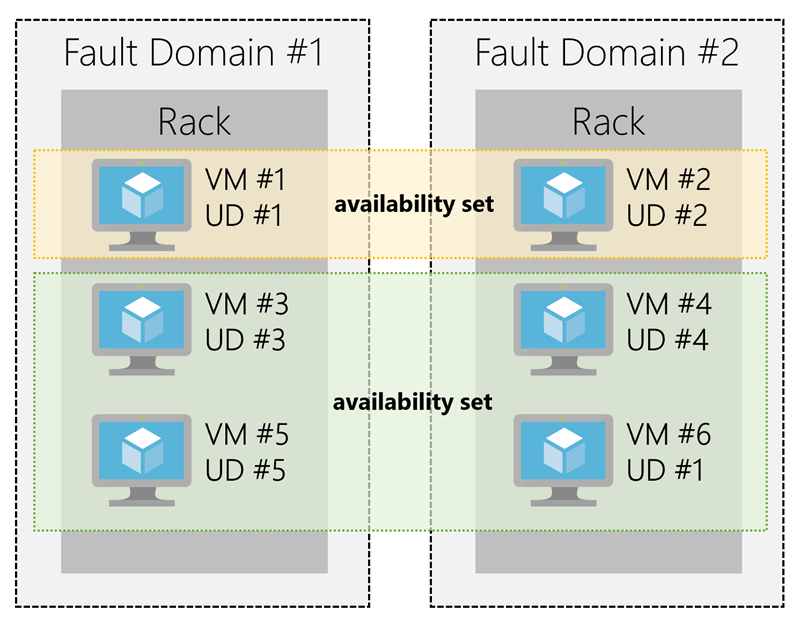
\includegraphics[width=7cm]{./Images/cap14/14.3.png}
\end{figure}

Grazie ai \textbf{Virtual Machine scale sets} è possibile creare e gestire insiemi di VM identiche e già bilanciate. Con i duplicati di macchine virtuali gli utenti devono configurare un servizio aggiuntivo per instradare le richieste tra istanze multiple dell'applicazione: il Virtual Machine scale sets può fare questo lavoro automaticamente. 

\subsubsection{\textbf{CONTAINERS}}
Un container è un ambiente di virtualizzazione per applicazioni in esecuzione. Anch'essi, come le macchine virtuali, eseguono su un sistema operativo host, ma a differenza delle VM non utilizzano un sistema operativo per le app che sono in esecuzione al loro interno. I container utilizzano pacchetti di librerie e componenti necessari ad eseguire l'applicazione e il sistema operativo che esegue il container.

\vspace{5mm}

Azure Batch permette di effettuare scheduling di operazioni a larga scala per la gestione di centinaia di macchine virtuali contemporaneamente. I task che può effettuare Azure batch sono:
\begin{itemize}
    \item avvio di un pool di VM;
    \item installazione di applicazioni e dati;
    \item identificazione di fallimenti;
    \item scaling del pool di risorse.
\end{itemize}
I servizi di containerizzazione di Azure si dividono in \textbf{Azure Container Instances}, servizi PaaS che offrono la possibilità di caricare le proprie applicazioni containerizzate con scaling automatico, e \textbf{Azure Kubernetes Service}, servizio di distribuzione completo per container o per architetture che contengono più container.

\textbf{Kubernetes} monitora le richieste delle applicazioni e scala di conseguenza grazie a servizi e ad API messe a disposizione degli utenti: l'infrastruttura è divisa in \textit{pods}: un pod rappresenta un Kubernetes cluster node, formato da più container, in questo modo è resistente ai fallimenti e gestisce i dati contenuti nel container automaticamente. Il traffico di rete è bilanciato tra i pod e limitato in base alle policy stabilite. I container aiutano a costruire architetture a microservizi.

È possibile migrare le applicazioni su container tramite AKS. Il controllo degli accessi avviene tramite Azure Active Directory e servizi di controllo degli SLA, tramite Open Service Broker for Azure. Gli step sono i seguenti:
\begin{itemize}
    \item Convertire un'applicazione esistente in uno o più container e pubblicare una o più immagini dei container nell'Azure Container Registry.
    \item Utilizzando il portale Azure o tramite riga di comando, distribuire i container in un cluster AKS.
    \item Azure AD controlla l'accesso ai cluster AKS.
    \item L'accesso ai servizi SLA viene gestito da OSBA.
    \item Opzionalmente, AKS può essere distribuito con un virtual network.
\end{itemize}

\subsubsection{\textbf{AZURE APP SERVICE}}
È una piattaforma PaaS progettata per ospitare applicazioni web-oriented di grado enterprise. Permette di soddisfare requisiti rigorosi di performance, scalabilità, sicurezza e conformità, utilizzando una piattaforma completamente gestita per la manutenzione dell'infrastruttura.

\vspace{5mm}

Azure App Service permette di sviluppare e distribuire applicazioni web, servizi background, backend e REST API in qualsiasi linguaggio di programmazione senza dover gestire l'infrastruttura. Supporta sia Windows che Linux, e permette deployment automatici da GitHub, Azure DevOps, e qualsiasi repository git. Questo modello PaaS permette ai clienti di focalizzarsi sul proprio sito e la logica delle API mentre Azure si occupa della parte dell'infrastruttura. Azure App Service gestisce la maggior parte delle decisioni infrastrutturali da prendere quando si ospitano le applicazioni sul cloud. Il deployment e la gestione sono integrate nella piattaforma, così come la sicurezza degli endpoint. Sono già integrate soluzioni di scaling automatico e load balancing. Può essere distribuito quasi ogni tipo di applicazione:
\begin{itemize}
    \item \textbf{Web Apps}: ASP.NET, ASP.NET Core, Java, Ruby, Node.js, PHP, Python.
    \item \textbf{API Apps}: REST-based web API utilizzando qualsiasi linguaggio.
    \item \textbf{Webjobs}: avvio di programmi o di script con funzionamento uguale ad un'applicazione o avvio schedulato.
    \item \textbf{Mobile Apps}: backend per app Android/iOS.
\end{itemize}

\subsubsection{\textbf{SERVERLESS COMPUTING}}
Il serverless computing è un ambiente di esecuzione ospitato sul cloud che esegue codice completamente indipendente dall'ambiente di host. Non è necessaria e non è permessa alcuna configurazione o manutenzione.

Grazie al \textbf{serverless computing} Azure si preoccupa di gestire le infrastrutture dei server e l'allocazione/deallocazione delle risorse basate sulla domanda: l'infrastruttura non è più un problema del consumer. Lo scaling e le prestazioni sono gestite automaticamente e la fatturazione viene fatta solo per le risorse utilizzate. Ci sono tre idee: astrazione dei server, scaling guidato dagli eventi e microfatturazione. 

L'idea di carichi di lavoro che si attivano con gli eventi funziona in quanto un evento può essere rappresentato con un trigger o con un timer, ad esempio un blocco di codice che deve essere eseguito ogni giorno a un determinato orario. Anziché scrivere un intero programma lo sviluppatore deve soltanto scrivere una funzione e stabilire dei trigger, e la piattaforma schedulerà automaticamente l'esecuzione della funzione e scalerà o meno in base alle richieste che arriveranno.

La microfatturazione è estremamente importante nel serverless computing in quanto non si va a pagare tutta l'infrastruttura ma si paga solo per quei pochi minuti o secondi in cui la funzione è in esecuzione. Se la funzione non viene chiamata da nessuno, non bisogna pagare.

\vspace{5mm}

Il serverless computing in Azure viene implementato in due modi diversi:
\begin{itemize}
    \item con le \textbf{Azure Functions}, che possono eseguire codice in qualsiasi linguaggio di programmazione moderno.
    \item con le \textbf{Azure Logic Apps}, che sono progettate sulla base di applicazioni web-based e permettono di eseguire funzioni attivate da servizi di Azure senza scrivere una riga di codice.
\end{itemize}
Le Azure Functions sono molto utili quando il servizio risiede nell'esecuzione di codice e non dipende da una particolare infrastruttura. Possono rispondere in pochissimo tempo e rispondono ad eventi via timer, via REST, o via messaggi da altri servizi Azure. Permettono di essere cost-effective perché le risorse vengono utilizzate solo quando le funzioni vengono chiamate, dopodiché vengono deallocate. Le Azure Functions possono essere stateless (di default) oppure stateful (dette anche \textbf{Durable Functions}), dove un contesto viene passato attraverso la funzione per tracciare l'attività principale. Le Azure Logic Apps sono simili alle Funzioni, entrambi vengono attivati da eventi, ma mentre le Funzioni eseguono codice le Logic Apps eseguono dei flussi di lavoro progettati per automatizzare degli scenari di business costruiti ad hoc da interazioni predefinite. La creazione di Logic Apps può avvenire tramite un visual designer sul portale di Azure o in Visual Studio. I workflow sono salvati in file JSON.

\begin{figure}[htb!]
    \centering
    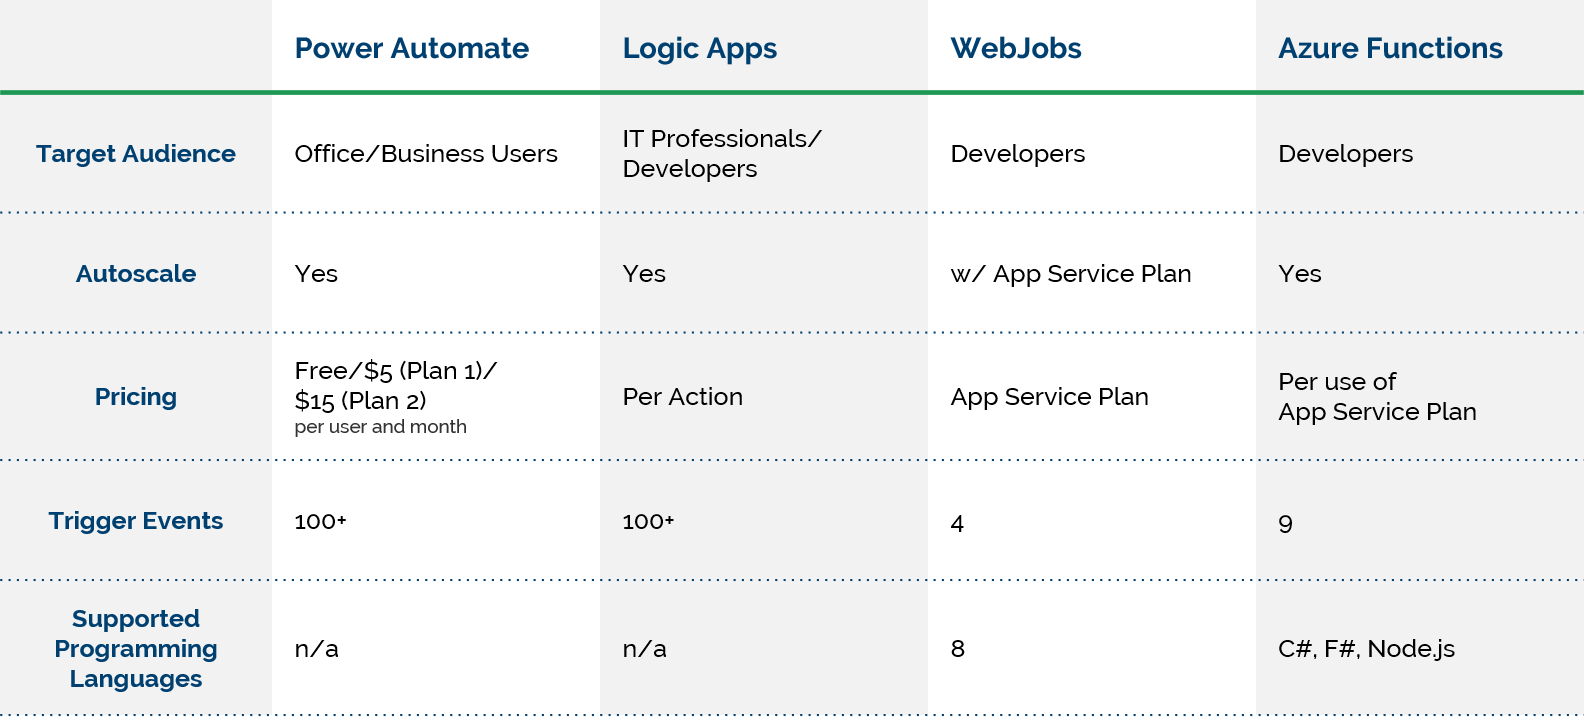
\includegraphics[width=9cm]{./Images/cap14/14.4.png}
\end{figure}

\subsection{Data Storage Options}
Archiviare i propri dati su Azure ha una serie di benefici, tra cui:
\begin{itemize}
    \item \textbf{backup e ripristino automatici}: mitigano il rischio di perdere i dati a causa di fallimenti o interruzioni.
    \item \textbf{duplicazione in tutto il mondo}: vengono effettuate delle copie in modo da proteggere i dati da qualsiasi tipo di errore o disastro.
    \item \textbf{supporto all'analisi dei dati}
    \item \textbf{supporto alla crittografia}
    \item \textbf{tipi di dati multipli}: Azure può salvare quasi tutti i tipi di dati esistenti, video, immagini, file di testo o file binari di grandi dimensioni, e supporta DMBS e database NoSQL.
    \item \textbf{Archiviazione di dati in dischi virtuali}: è possibile salvare i dati fino a 32 TB in dischi virtuali, utili nel caso di file molto pesanti o di simulazioni di modelli 3D.
    \item \textbf{Dato strutturati e semi-strutturati}: un dato viene chiamato strutturato quando è conforme a un determinato schema, ovvero quando due dati diversi hanno le stesse proprietà o campi. I dati strutturati si trovano ad esempio in un database fatto di righe e colonne. I dati semistrutturati non seguono tutti lo stesso schema e spesso vengono utilizzati per definire una gerarchia di dati. Ci si riferisce ai dati strutturati anche come dati non relazionali.
\end{itemize}
\textbf{Azure SQL Database} è un DaaS (Database as a Service) basato sulla versione piu recente di Microsoft SQL Server Database. Ha prestazioni molto elevate e un livello di sicurezza alto. È possibile migrare database SQL Server già esistenti su Azure database in pochissimo tempo, grazie all'assistente di migrazione di Microsoft.

\textbf{Azure Cosmos DB} è un servizio distribuito di database che supporta dati non strutturati e permette quindi di costruire applicazioni always on che hanno la capacità di visualizzare dati che cambiano continuamente.

\textbf{Azure Blob Storage} è un servizio di archiviazione che supporta dati non strutturati: i blob sono facilmente scalabili e le applicazioni lavorano con essi pressoché allo stesso modo di come lavorano con i dati su un disco, con le normali operazioni di lettura e di scrittura. Può gestire migliaia di upload simultanei, log che crescono costantemente e vi si può accedere da qualsiasi locazione a patto di avere una connessione ad Internet. Un blob può contenere GB di dati binari e può rappresentare qualsiasi tipo di dato. I blob vengono utilizzati anche per salvare i backup in caso di disaster recovery e per l'archiviazione. Ogni macchina virtuale può salvare circa 8 TB di dati in formato blob.

\textbf{Azure Files} offre un servizio di gestione file nel cloud accessibile via il protocollo standard Server Message Block (SMB), che assicura anche che i dati siano criptati. Le applicazioni che sono in esecuzione su Azure condividono un file share per accedere ai dati. È molto utile per condividere file ovunque nel mondo.

\textbf{Azure Queue Storage} è un servizio per archiviare un grande numero di messaggi a cui vi si può accedere in qualsiasi momento. Può essere utilizzato per costruire applicazioni flessibili e funzioni separate per aumentare la durabilità delle componenti con carichi di lavoro molto elevati. Le componenti con basso accoppiamento in un'applicazione possono scalare indipendentemente una dall'altra. Azure Queue Storage fornisce un sistema a coda asincrona di messaggi per le comunicazioni tra le componenti delle applicazioni, a prescindere se queste siano in esecuzione sul cloud oppure on-premise. 

\textbf{Azure Disk Storage} fornisce i dischi per le macchine virtuali, per le applicazioni e per altri servizi che necessitano di spazio di archiviazione. Permette di archiviare permanentemente i dati e di accedervi ogni qualvolta ce ne sia bisogno. I dischi possono essere gestiti sia dall'utente che direttamente da Azure. I dischi vengono forniti in diverse dimensioni e livelli di performance, da dischi a stato solido (SSD) a classici hard disk (HDD).

\begin{figure}[htb!]
    \centering
    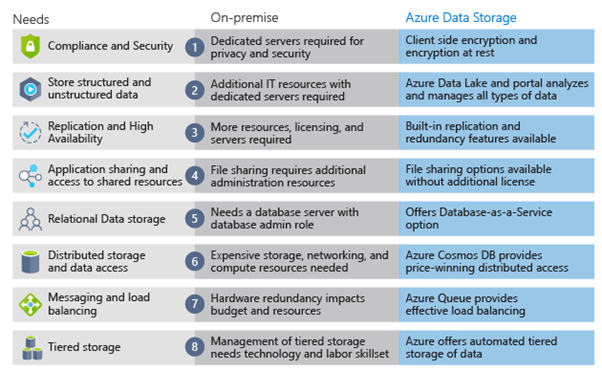
\includegraphics[width=12cm]{./Images/cap14/14.5.png}
\end{figure}

\subsection{Networking Options}
Quando si parla di availability per un sito, ci si riferisce a quanto tempo il servizio riesce ad essere in esecuzione senza essere interrotto. High availability, quindi alta disponibilità, indica un servizio che esegue da molto tempo senza fermarsi. Con resilienza intendiamo l'abilità di un sistema di essere attivo durante condizioni anormali (disastri naturali, manutenzioni di sistema, picchi nel traffico). Un load balancer distribuisce il traffico attraverso i vari sistemi presenti in un pool di risorse: il suo scopo è quello di raggiungere un'alta disponibilità e una forte resilienza. \textbf{Azure Load Balancer} supporta bilanciamento del traffico in uscita e in entrata del sistema, fornisce bassa latenza e altro throughput, e scala milioni di flussi per tutte le trasmissioni che avvengono tramite TCP e UDP. La cosa più importante è che non occorre alcuna infrastruttura o software per la manutenzione.

\textbf{Application Gateway} è un load balancer progettato per le applicazioni web. Il bilanciamento del traffico a livello 7 della pila ISO/OSI offre una serie di vantaggi:
\begin{itemize}
    \item \textbf{Cookie affinity}: per mantenere attiva la sessione dell'utente sullo stesso server.
    \item \textbf{SSL termination}: gestisce i certificati SSL e passa il traffico non criptato ai server di backend per evitare un overhead dovuto alla cifratura e alla decifratura dei messaggi. Supporta anche la crittografia end-to-end per le applicazioni che la richiedono.
    \item \textbf{Web Application Firewall (WAF)}: monitora dettagliatamente i tentativi di attacchi al sistema e li salva nei log.
    \item \textbf{URL rule-based routes}: instradamento del traffico basato su pattern URL, con indirizzo IP di partenza, di destinazione, e porta. Molto utile quando si installa un Content Delivery Network.
\end{itemize}



\begin{comment}

\begin{figure}[htb!]
    \centering
    \includegraphics[width=9cm]{./Images/cap14/14..png}
\end{figure}

\end{comment}

\section{Learning Check}
\begin{enumerate}
    \item Cos'è Microsoft Azure?
    \item Quali sono i servizi offerti per l'hosting di applicazioni?
    \item Quali sono i servizi offerti per il data storage?
    \item Qual è lo scopo di avere diverse regioni/geografie/availability zones?
    \item Come possono essere gestiti i servizi?
    \item Per ogni servizio fornito da Azure (inclusi la gestione, la fatturazione, ecc.) fornisci un collegamento con le architetture viste nelle lezioni precedenti.
\end{enumerate}

 